\section{Results}
\label{sec:results}
\subsection{Algorithm Convergence}
\label{sec:convergence}
\begin{figure}[H]
  \centering
  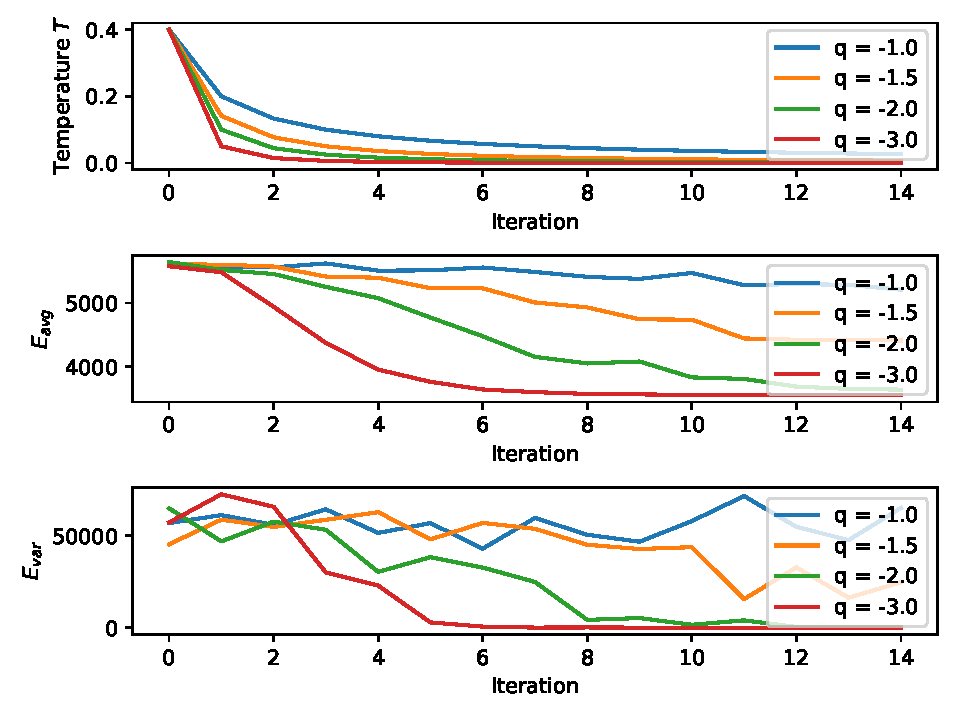
\includegraphics[width=0.8\linewidth]{results/convergence-8h-day.pdf}
  \caption{Temperature, average energy and energy variance for an 8-hour work day. Low variance can be used as a stopping criterion (cf. \Cref{sec:theory}).}
\end{figure}
\begin{figure}[H]
  \centering
  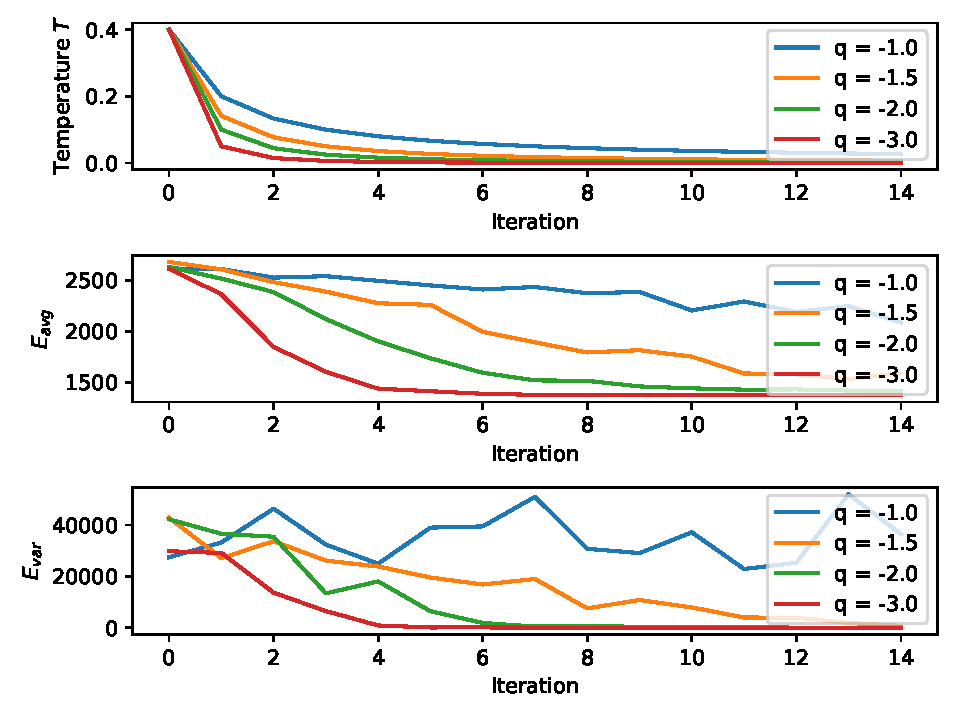
\includegraphics[width=0.8\linewidth]{results/convergence-14h-day.pdf}
  \caption{Temperature, average energy and energy variance for a 14-hour work day.}
\end{figure}

\subsection{Runtime Performance}
\label{sec:runtime}
The following benchmarks were all accumulated on an x86\_64 Intel\textregistered \, i7-5600U CPU running at \SI{2.6}{\giga\hertz} verified through 3 individual runs, keeping parameters consistent along them.

\begin{figure}[H]
  \centering
  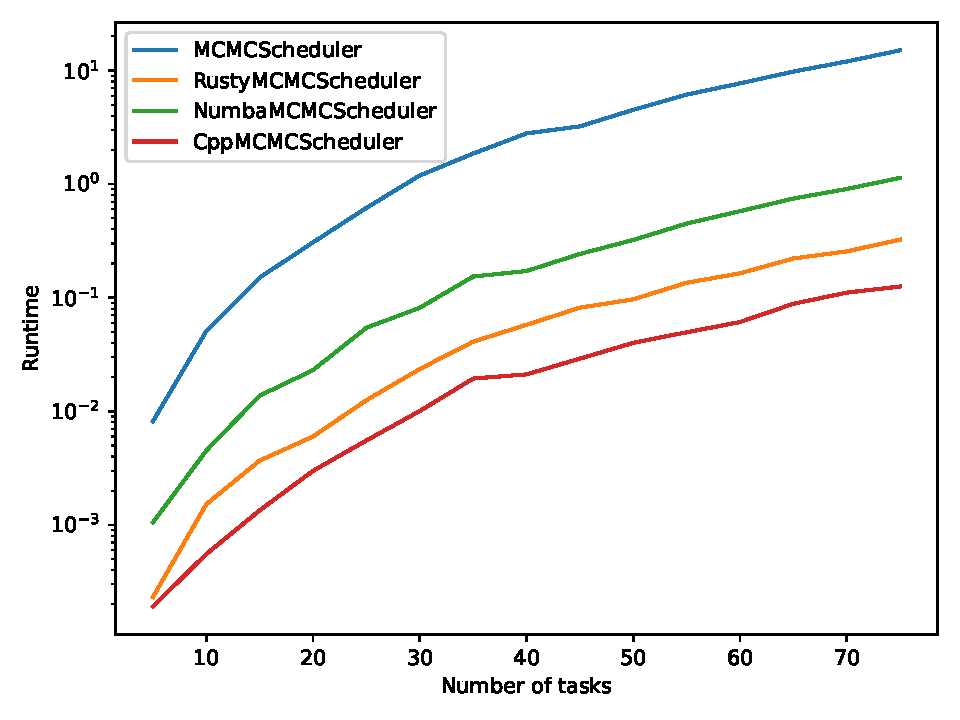
\includegraphics[width=0.7\linewidth]{results/complexity.pdf}
  \caption{Complexity plot}
\end{figure}

\begin{table}[H]
  \vspace{0.5cm}
  \centering
  \caption{Runtime Comparison of the different implementations run on the same scenarios. Each runtime is given as the average over three runs.}
  \begin{tblr}{
    colspec={llr},
    row{2,3} = {bg=azure9},
        row{4} = {bg=violet9},
        row{5} = {bg=cyan9},
      }
    \hline
    \bf Implementation & \bf Language & \bf Runtime / seconds \\
    \hline
    MCMCScheduler      & Python & 31.3887 \\
    NumbaMCMCScheduler & Python & 1.9335 \\
    \hline
    RustyMCMCScheduler & Rust & 0.4034 \\
    \hline
    CppMCMCScheduler   & C++ & 0.4062
    \hline
  \end{tblr}
  \label{table:runtime}
\end{table}

Regarding the table above, one should note that the Numba compilation time was approximately 3.2 seconds, which takes place once for each Python process.

\begin{table}[H]
  \centering
  \caption{Profile obtained by running \mintinline{bash}{inv profile-scheduler | grep purepython.py}.}
  \begin{tabular}{rrrrrll}
    \hline
    \bf Ncalls & \bf Total & \bf / call & \bf Cum. & \bf / call & \bf Filename:line & \bf Function     \\
    \hline
    1          & 0.000     & 0.000      & 14.236   & 14.236     & purepython:142    & schedule         \\
    10         & 0.209     & 0.021      & 14.235   & 1.424      & purepython:123    & mcmcSweep        \\
    36010      & 1.144     & 0.000      & 13.784   & 0.000      & purepython:97     & computeEnergy    \\
    2196671    & 5.391     & 0.000      & 11.353   & 0.000      & purepython:41     & spreadTasks      \\
    1006332    & 1.389     & 0.000      & 1.842    & 0.000      & purepython:27     & generateNextSlot \\
    2196610    & 0.798     & 0.000      & 0.972    & 0.000      & purepython:108    & <genexpr>        \\
    2196610    & 0.384     & 0.000      & 0.384    & 0.000      & purepython:106    & <genexpr>        \\
    36000      & 0.082     & 0.000      & 0.217    & 0.000      & purepython:83     & permuteState     \\
    36011      & 0.046     & 0.000      & 0.124    & 0.000      & purepython:19     & startingSlot     \\
  \end{tabular}
\end{table}
